\chapter{Introduction}
The paper studies the Qur'\=an through the use of scientific computing, and the new perspective and methodology it brings will therefore be of interest, respectively, to researchers from Islamic studies, and researchers from the field of Statistics, Machine Learning, and Data Science. Thus, it is necessary to provide the essential background on Quranic studies to give more context on the rationales of the paper. 
\section{Background}
The Qur'\=an or \arb[trans]{al-qur'An} \arb{al-qur'An} meaning \textit{the recitation}, the holy book of Islam, is revered by 1.9 billion (according to 2020 projection of \shortciteA[p.~13]{pewresearch}) Muslims across the globe as the literal words of God. Muslims believed that the Qur'\=an was gradually revealed (Qur'\=an 25:32) to Prophet Muhammad \arb{\arbmark{slm}} through angel \arb[trans]{jibrIl} \arb{jibrIl} or Gabriel (Qur'\=an 2:97). The Qur'\=an contains 77,429 Arabic words in total, which covers only 56 percent of the Greek New Testament which has 138,020 words in total \cite[p.~11]{sinai2017}. 

The Qur'\=an is divided into \textit{s\=urahs} \arb{sUr} which are the equivalent of chapters, each containing \arb[trans]{'ayAt} \arb{'ayAt} (meaning \textit{signs}), which are the equivalent of verses. The \textit{s\=urahs} \arb{sUr} are not arranged in chronological order as in the Bible's books and chapters, but rather arranged in monotonically decreasing length of number of verses after the first \textit{s\=urah} \arb{sUraT} (\textit{see} Figure \ref{fig:ayah_word_count}). The \textit{s\=urah} \arb{sUraT} of the Qur'\=an can be categorized into two types: the \arb[trans]{makkiyyaT} \arb{makkiyyaT} (Meccan) and \arb[trans]{madaniyyaT} \arb{madaniyyaT} (Medinan). The categories refer to the geographical location of where the \textit{s\=urah} \arb{sUraT} was revealed. Figure \ref{fig:ayah_word_count} shows the grouping of the \textit{s\=urahs} \arb{sUr}. Note that some of the \textit{s\=urahs} \arb{sUr} have mixed geographical locations\footnote{\textit{see} list of the location in \url{https://tanzil.net/docs/revelation_order}}, that is, a few of the \arb[trans]{'ayAt} \arb{'ayAt} in it were revealed in other geographical location apart from the geographical location of the rest of the \arb[trans]{'ayAt} \arb{'ayAt}. Therefore, the categorization in Figure \ref{fig:ayah_word_count} highlights the geographical location of the majority of the \arb[trans]{'ayAt} \arb{'ayAt} in the \textit{s\=urah} \arb{sUraT}.

\begin{figure}[!b]
    \centering
    \includegraphics[width=\textwidth]{img/plot1.pdf}
    \caption{Statistics of the words and \arb[trans]{ayAt} \arb{ayAt} (verses) of the Qur'\=an}
    \label{fig:ayah_word_count}
\end{figure}

The Qur'\=an (meaning \textit{the recitation}) was revealed \textit{orally} by angel \arb[trans]{jibrIl} \arb{jibrIl} to Prophet Muhammad \arb{\arbmark{slm}} and passed onto other believers through oral tradition (reciting the Qur'\=an to students repeatedly so as to memorize it, instead of writing it down and let the believers read it and memorize it). Memorizing 77,429 Arabic words of the Qur'\=an through oral transmission can be a difficult task, but what aids this memorization is the rhythm feature of the Qur'\=an. According to one Orientalist, \citeA{sinai2017}, "rhyme, however, or rather a periodically recurrent word-final assonance, is a feature of the Qur'\=an throughout, and it naturally partitions the \textit{s\=urah} \arb{sUraT}." Indeed, because of this feature, it makes it easy to memorize the entire Qur'\=an, and the one who do so is called \arb[trans]{hafi.z} \arb{hafi.z} meaning \textit{one who remembers} or \textit{keeper}. Qur'\=an memorization contest is a common event in Muslim countries, the Philippine embassy has hosted one in 2022 in Saudi Arabia \cite{mb2022}.

According to the Muslim tradition, the oral transmission of passing the Qur'\=an from a \arb[trans]{hafi.z} \arb{hafi.z} to new believers was gradually put into writings as requested by the believers themselves. The idea was brought up after the battle of Yamama, where many of the Muslims who died were \arb[trans]{qurrA'} \arb{qurrA'} (\textit{the one who properly recite the Qur'\=an}), and so fearing that their numbers will reduce in other battle fields, Umar ibn al-Khattab \arb{`umaru bnu 'l-xa.t.tAb} (who became the second caliph) suggested to the first caliph, Ab\=u Bakr 'Abd All\=ah ibn 'Ab\=i ibn 'Ab\=i Qu\d{h}\=afa, \arb{'abU bakriN `abdu 'l-lAhi 'ibni 'abiY qu.hAfaTa} or short for Ab\=u Bakr \arb{'abU bakr}, to collect the Qur'\=an into writing. Ab\=u Bakr then authorized Zaid ibn Thabit \arb{zaydi bni _tAbitiN} for the task. According to Zaid, he started collecting from the leafless stalks of the date-palm tree and from the pieces of leather and hides and from the stones, and from the chests of men (who had memorized the Qur'\=an, i.e. the \arb[trans]{hafi.z} \arb{hafi.z})\footnote{\textit{see} \url{https://sunnah.com/bukhari:7191}}. Long story short, the effort was finally codified by the third caliph, Uthman ibn Affan \arb{`u_tmAnu bnu `affAn} in the year 645 CE, which was then recopied and distributed to the different regional capitals of the early Islamic empire of that time. The rest of the copies outside this codification were then burned\footnote{\textit{see} \url{https://sunnah.com/bukhari:4987}} down in order to have one standard Qur'\=an. The Qur'\=an nowadays is therefore assumed to be based on Uthmanic codex because of the story mentioned. That is, if indeed Uthman has ordered to burn other copies of the Qur'\=an outside his codification, then what's left should only be based on his codex or archetype, and that should only be the inherited codex of the Muslims today.

The Qur'\=an is believed by the Muslims to have been preserved since it was first recited by angel \arb[trans]{jibrIl} \arb{jibrIl} or Gabriel to the Prophet \arb{\arbmark{slm}}. Many orientalists had been skeptic about this claim, for example, John Wansbrough theorized that the Qur'\=an was collected over a 200-year period \cite<\textit{see}>[p.~101]{wansbrough2004} after the death of the Prophet \arb{\arbmark{slm}}, instead of within a few years after the death of the Prophet \arb{\arbmark{slm}}. However, recent findings through radiocarbon dating brings forward strong evidence of potential preservation of the whole Qur'\=an, which the Muslims believed to be so. For example, the Birmingham Qur'\=an manuscript discovered in 2015 is dated to be between 568 and 645 CE with 94.5\% accuracy, making it among the oldest Qur'\=anic manuscript in the world \cite<\textit{see} >{bu2015}. Its predicted range of years intersects with the lifetime (570 to 632 CE) of the Prophet \arb{\arbmark{slm}}. What is interesting is that the Birmingham Qur'\=an is consistent with the Qur'\=an today, word-by-word and letter-by-letter\footnote{The orthography of the Arabic letters in the early days had no diacritics and were written in its basic consonantal skeleton. That is, Arabic orthography and grammar were in their nascent when the Qur'\=an was revealed, and therefore has to adjust and catch up, to capture and preserve the proper recitation of the Qur’an.}, see Figure \ref{fig:birmingham}. This is indeed another evidence that the Qur'\=an today was codified by Uthman since the discovery of the Birmingham Qur'\=an manuscripts have confirm it. In addition to this, the Sana'a Palimphest is also among the oldest Qur'\=an radiocarbon dated to be between 578 CE and 669 CE with 95\% accuracy \cite{behnam2010}, which according to \citeA{sinai2017}, "neither does the edited portion of the Sana'a palimpsest offer evidence for additional or missing verses or for a divergent verse order within the \textit{s\=urahs} \arb{sUr}." Given these discoveries on the recent Quranic manuscripts, the claim of \citeA[p.~101]{wansbrough2004} is now untenable \cite<\textit{see}>{sinai_2014}.

\begin{figure}[!b]
    \centering
    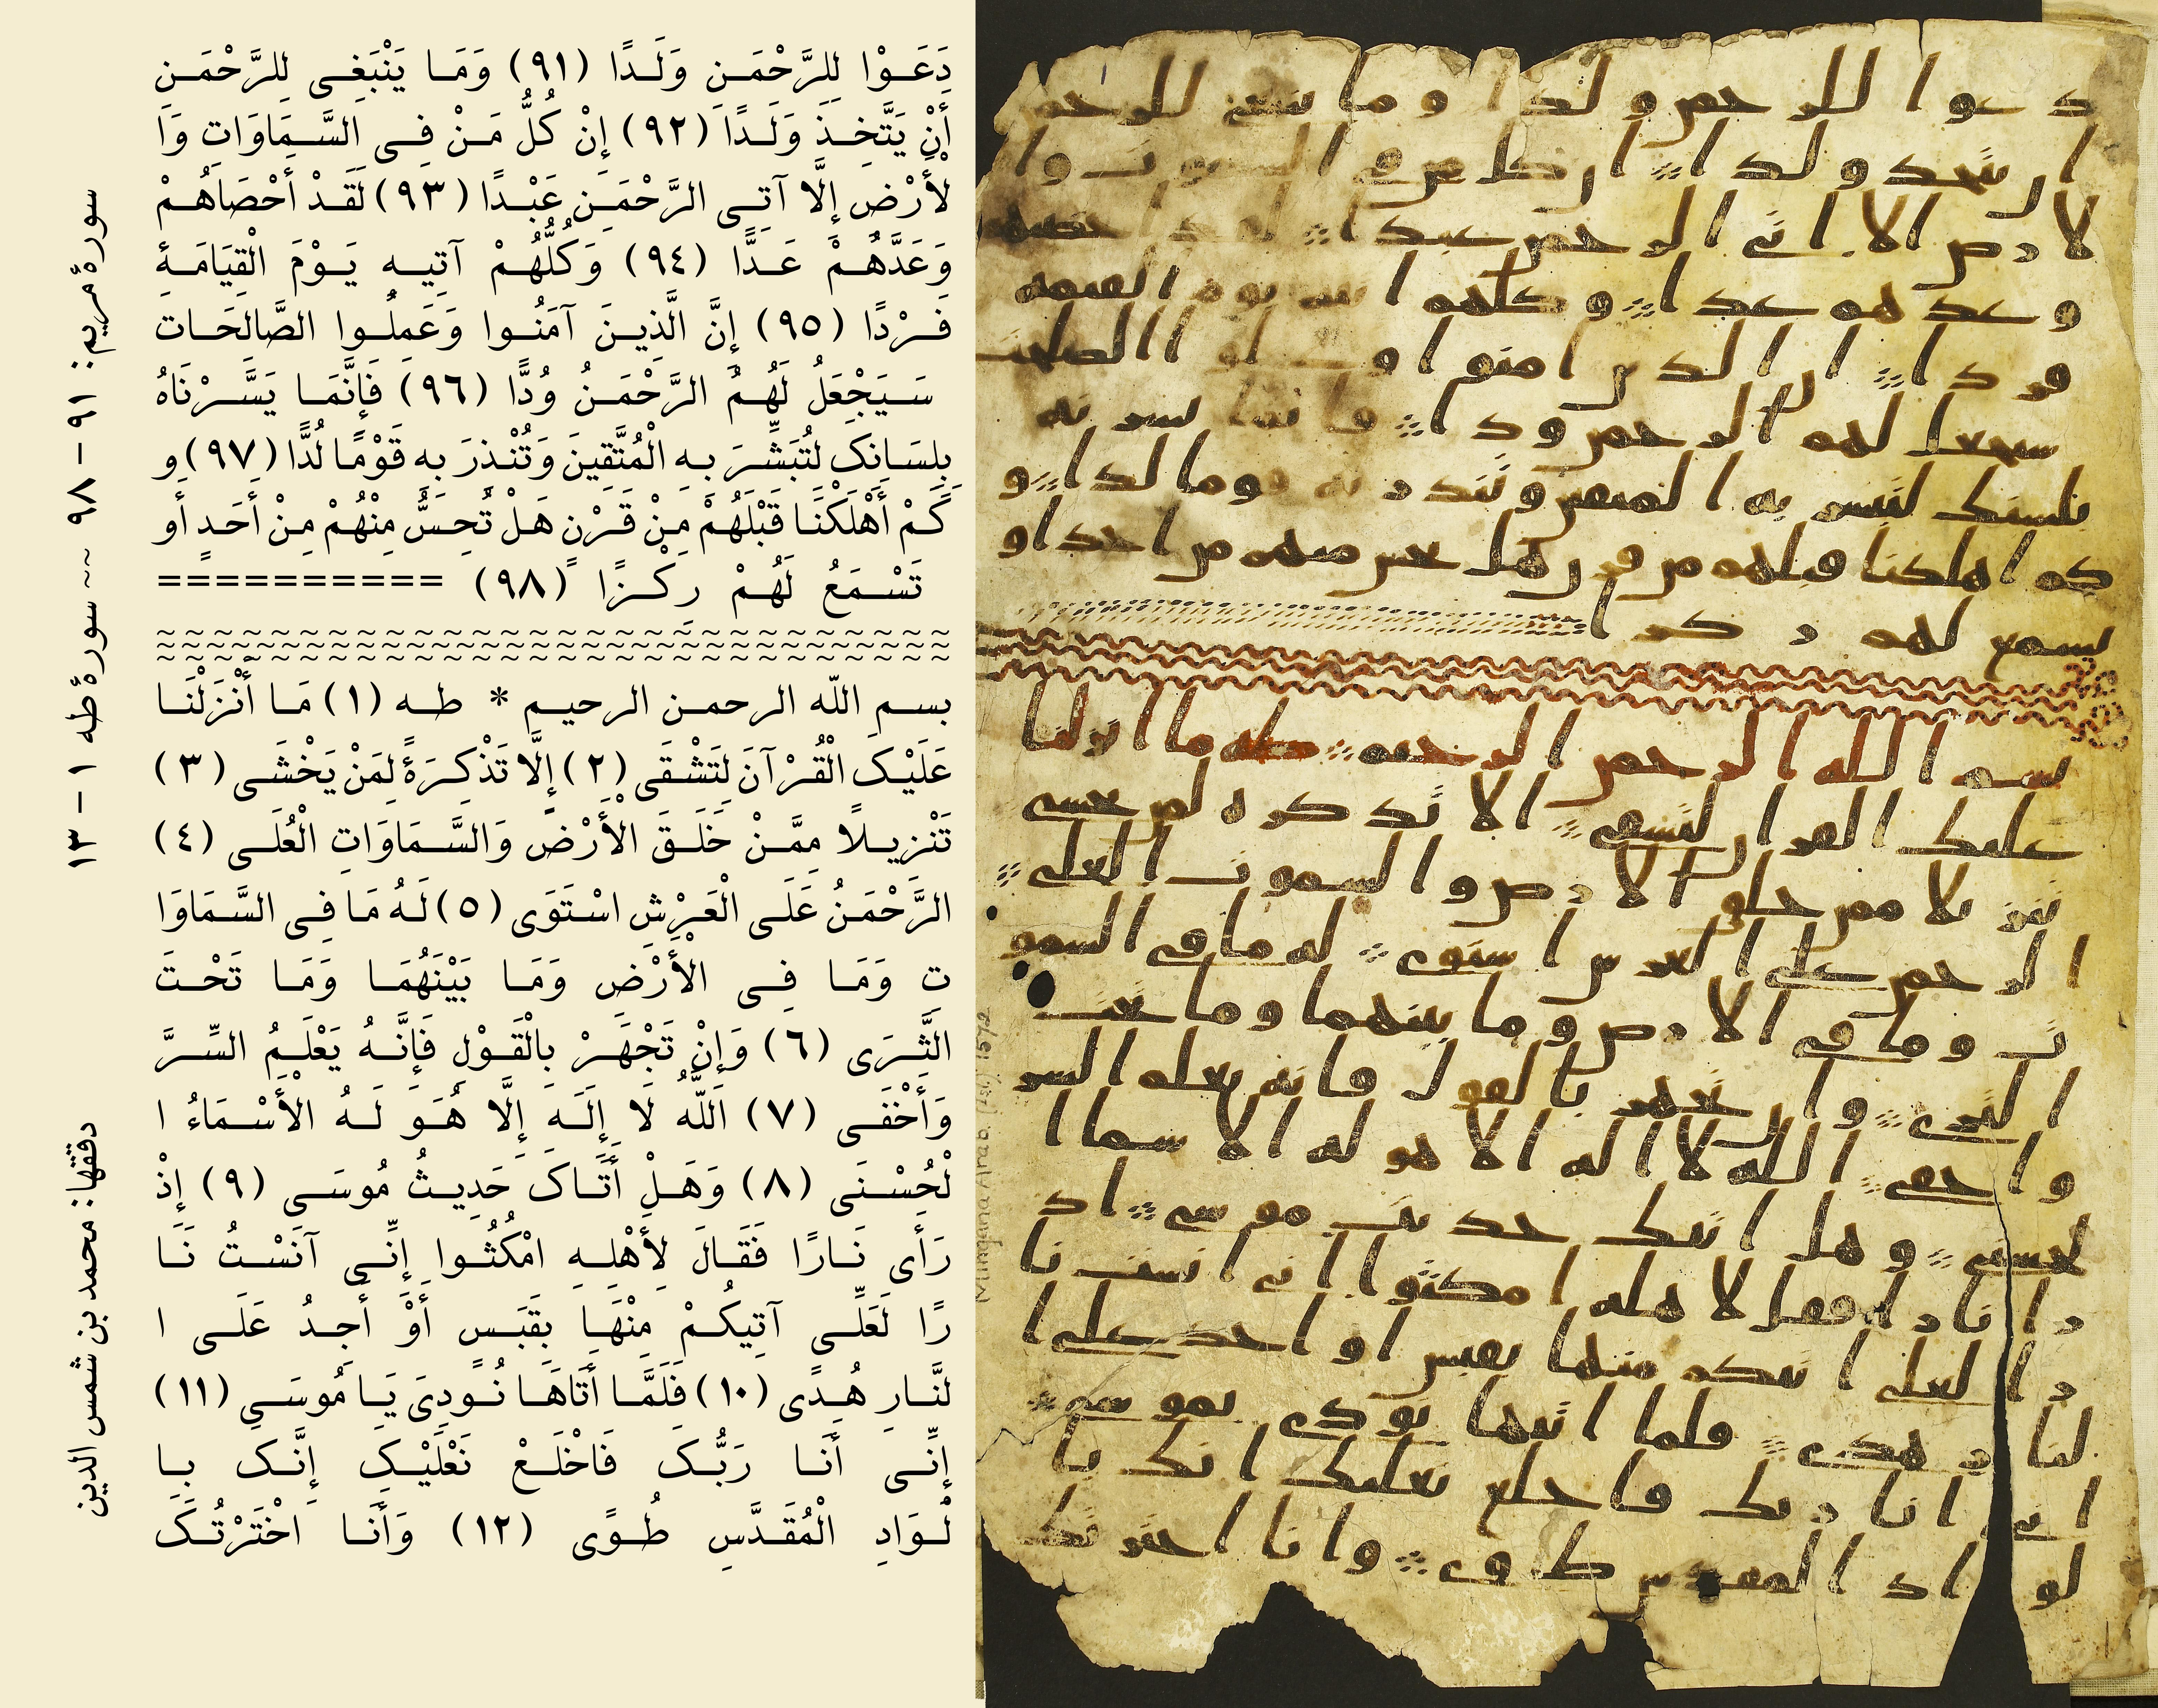
\includegraphics[width=\textwidth]{img/birmingham.jpg}
    \caption{20th Century Qur'\=an (left) in its fully featured orthographies vs Birmingham Qur'\=an dated between 568 and 645 CE (right) in its basic consonantal skeleton. Image from \protect\citeA{wikibirmingham}.}
    \label{fig:birmingham}
\end{figure}

One likely reason as to why the scribes were able to preserve the Qur'\=an in the two folios of the Birmingham Qur'\=an manuscripts follows from the fact that the Qur'\=an is firstly memorized before it was decided to be written. So that, the \mbox{Topkapi} manuscripts that contain 99\% (only 23 verses missing)---dated around 701 to 750 CE \cite{karatay1962}\footnote{\textit{see also} \url{https://corpuscoranicum.de/en/manuscripts/1977/page/1-410?sura=1&verse=1}}, that is, around 69 to 118 years after the death of the Prophet \arb{\arbmark{slm}}---of the Qur'\=an today was likely partly written from memory. This is possible since the Qur'\=an possesses a rhytmic feature (that aids with memorization) that naturally divides its verses or \arb[trans]{'ayAt} \arb{'ayAt}, and that the Qur'\=an memorization competition is still held to this day \cite<as in the example of >{mb2022}, apart from the fact that it needs to be recited (any chapter after the first chapter of the Qur'\=an according to the choice of the worshipper) every prayer from memory. Bottomline, there are many avenues for Qur'\=an recitation from memory, and these have helped in its preservation. Moreover, since there are no significant evidence of insertion or malicious intention on addition or revision in all of the extant Qur'\=anic manuscripts so far, some Orientalists came up with other theories of insertions on the basis of the literary style of the Qur'\=an, see for example \citeA[p.~92]{sinai2017}, where verse 102 of \arb[trans]{sUraT 'l-.sAffAt} \arb{sUraT 'l-.sAffAt} or The Chapter of \textit{Ranged in Rows} is theorized as addition because it is longer compared to other verses in the said chapter, refer to \citeA[p.~92]{sinai2017} for his other reasonings. Nonetheless, the Qur'\=an is indeed stable based on the extant manuscripts.

Furthermore, the vastness of the early Islamic empire meant that different Muslim regional capitals have covered populations with different Arabic dialects, and so to accommodate these differences, Muslims believed that there were seven variant readings of the Uthmanic codex. Variant readings are defined as different pronunciations of the same word, in this case seven Uthamnic Qur'\=an for seven different pronunciations. The \arb[trans]{.hadI_t} \arb{.hadI_t} or \textit{narration} comes from Ubayy ibn Ka'b \arb{'ubayyi bin ka`b} who reported\footnote{source: \url{https://sunnah.com/muslim:821a}} that the Prophet \arb{\arbmark{slm}} was near the tank of Banu Ghifar that \arb[trans]{jibrIl} \arb{jibrIl} or Gabriel came to him and said: "... Allah has commanded you to recite the Qur'\=an to your people in \textit{seven dialects}, and in whichever dialect they would recite, they would be right." Recent work of \citeA{sidky2020} shows that the material evidence on the regional variants is in remarkable agreement with well-attested written variants documented in the traditional Muslim literature.

Muslim and non-Muslim scholars alike have been extremely interested in understanding the unique literary characteristics of the Qur'\=an. As mentioned earlier, unlike other books like the Bible (arranged in chronological order), the Qur'\=an does not follow any obvious organization. In addition to this, a \textit{s\=urah} \arb{sUraT} does not fit the exact definition of a chapter. Indeed, the name attached to a \textit{s\=urah} \arb{sUraT} is often decided as the unique entity mentioned in the said \textit{s\=urah} \arb{sUraT}, its main purpose is to help early Muslims distinguish which \textit{s\=urah} \arb{sUraT} they are talking about, this is contrary to the chapter name where the associated name is obviously the main topic of the chapter. Further, as described by \citeA{sinai2017}, "... the compositional unity of the long surahs located at the beginning of the corpus is anything but obvious: at least at first sight, they can appear a flit back and forth between different topics in a largely haphazard manner. This impression is not limited to Western readers: even pre-modern Muslim scholars have often approached their scripture as a quarry of unconnected verses and groups of verses that bear little intrinsic relation to what precedes and follows." It wasn't until \citeA{Neuwirth_2007}, that the compositional unity of the Qur'\=an can be observed in tighter literary unities, as \citeA{Neuwirth_2007} showed that the many of these texts display a tripartite structure and are often constructive around a narrative middle part \cite{sinai2017}. Samples of the organizational style of the Qur'\=an was shown in \citeA[p.~88]{sinai2017}.

\section{Rationale of the Study}\label{sec:rationale}
Attempts at understanding the Qur'\=an by Qur'\=anic scholars were mostly done through manual process, that is, studying the scriptures by going through its content one-at-a-time manually. However, with the advent of computers some researchers have started using it to aid in their research. The first known to have used computers for studying the Qur'\=an was likely Rashad Khalifa in 1968\footnote{\textit{see} \url{https://www.masjidtucson.org/quran/miracle/a_profound_miracle_sura68nun133.html}}, where he studied the significance of the mysterious initials at the beginning of some \textit{s\=urahs} \arb{sUr}. Rashad uploaded the Qur'\=an into his computer by transliterating the Arabic letters and other Qur'\=anic orthographies into Roman letters and symbols that the computer can easily parse. This approach of using computers to find new insights is more common in the field of science, and it was new for the field of Qur'\=anic studies.

Indeed, to proceed with the use of scientific computing, the Qur'\=an will be treated as the data that needs to be analyzed using what is called Natural Language Processing (NLP), a branch of Machine Learning (ML) that aims to understand natural language, such as Arabic. To instruct the computer to do Statistical analyses, ML, or NLP, one needs to use a \textit{software application} or a formal language called \textit{programming language}. There are several programming languages that the computer can understand. The popular one for researchers in the field of science are Python, R, and sometimes Julia \shortcite{Julia2017}. These programming languages will be used to construct instructions for computer. Therefore, if the data is the Qur'\=an, then obviously there should be a way to interface with the Qur'\=an using any of these programming languages, or to upload it and encode the Arabic letters into something that can be easily parsed by the computer, like what Rashad Khalifa did. There are, however, som programming languages with libraries or packages for interfacing with the Qur'an, and this is true for Python, R, and Julia. For this study, Julia programming language is used since its library for interfacing the Qur\=an, QuranTree.jl\footnote{\textit{see} \url{https://alstat.github.io/QuranTree.jl/stable/}}, is based on Tanzil\footnote{\url{https://tanzil.net/download/}} for the Qur\=anic Arabic texts, and \citeA{dukes-habash-2010-morphological} for morphological annotation, which both R and Python's libraries for Qur\=an does not have morphological annotation from \citeA{dukes-habash-2010-morphological}.

Machine Learning is a branch of Artificial Intelligence that aims to characterize data (in this case Arabic texts) by learning its features. These learned features are captured by an artifact called \textit{model}. Basically, it is a model of some real data, meaning if there is a good representation of this real data, it is the model that has captured/learned/characterized the characteristics of the said real data. Therefore, a model is not exactly the real data, but an estimate of the characteristics of that data. To help understand this, and relate it to the fashion industry, which the author assumes most readers will be familiar with, a model in the fashion industry aims to capture the characteristics of the target customers, so for a clothing company, they hire a model which has the best features of their target customers. Hence, they hire Asian models to target Asian customers. So that, when these models wore the clothes sold by the said company, the potential customer will more or less be able to relate to the model, and be able to imagine themselves wearing that same clothes as well, which help them incline to buying the said clothing. The model therefore does not necessarily have the looks of every target Asian customer, but at least in terms of height, skin tone, hair, and other common Asian features, the model will likely have it. The question now is, what are the benefits that this model can bring to the clothing company? Well, the clothing company will be able to create products that are tailored to their Asian customers using the said model, since the company will have the right baseline measurements needed. Relating this analogy to the technical concept discussed earlier, you can think of the target customer as the
real data, and the model as the same technical term use in Machine Learning and Statistics, but this time this technical model is expected to capture the characteristics of the real data analogous to fashion model that is expected to capture the characteristics of the target customer. This Statistical or Machine Learning model brings the following benefit: researchers will be able to study the real data by simply using the model to answer questions that are not available in the sampled real data.

\section{Objectives}\label{sec:objectives}
The objective of the paper is to answer the following research questions:
\begin{enumerate}
    \item What are the thematic themes of the surah that can be extracted by a Statistical and Artificial Intelligence (AI) models?

    \item What other insights can be extracted by AI and how it compares or supplements the related findings from Muslim's traditional sources?
    
    \item How this combination of AI and Muslim's traditional literatures help in understanding the Qur\=an?
\end{enumerate}
\section{Significance of the Study}\label{sec:significance}
While the Qur'\=an has been extensively studied by Muslims and non-Muslims scholars alike, especially in the topic of Meccan and Medinan surahs, there is still a lot to uncover from the perspective of Computational Statistics. Hence, the significance of this study is that it brings forward new ways of extracting insights from the Qur'\=an by leveraging Computations, Statistics, Machine Learning, and AI, that is still in its early stage in the field of Qur'\=anic Studies. Therefore, this new perspective or process of studying the scripture not only aids the scholars of the Islamic Studies, but may also contribute indirectly to community development and policy makers who use Qur'\=an as part of their decision making.
\section{Scope of the Study}
The paper will cover all chapters of the Qur'\=an in the analyses. It will also not delve too much into the tafsir of each of the verses in the analyses, but will do on a few that may need further context.
\section{Thesis Organization}
The paper is organized as follows: Chapter 2 will discuss the related literatures, Chapter 3 will discuss the methodology, Chapter 4 will present the results and discussions, and finally Chapter 5 will contain the conclusion and recommendation. The references and appendices are placed after the Chapter 5.